\documentclass{acm_proc_article-sp}

\usepackage{makeidx}  % allows for indexgeneration
\usepackage{listings}
\usepackage{amsmath}
\usepackage{graphicx}
\usepackage{subfigure}
\usepackage{color}
\usepackage{url}

\newcommand{\FIXME}[1]{{\color{red}\textbf{FIXME: #1}}}

\title{A Pacman Game
\numberofauthors{2}
\author{
\alignauthor Ben Lickly \\
       \affaddr{University of California, Berkeley}\\
       \affaddr{Berkeley, CA, USA} \\
       \email{blickly@eecs.berkeley.edu}
\alignauthor Darren Kuo \\
       \affaddr{University of California, Berkeley}\\
       \affaddr{Berkeley, CA, USA} \\
       \email{darrenkuo@eecs.berkeley.edu}
}
}


\begin{document}
\maketitle

\begin{abstract}
\ldots
\cite{ZombieRun}
\end{abstract}

\section{Introduction}
\section{Background}
Augmented reality refers to a view of the physical world that has been
augmented with additional computer-generated information, creating a sort of
hybrid between virtual reality and the real world. Existing applications
include games, sightseeing guides, navigation aids, and automatic translators.

Recent years have seen the success of a new class of video games with new
methods of input, such as Dance Dance Revolution, Nintendo Wii, Playstation
Move, and Microsoft Kinect. We see Augmented Reality games where players leave
their game machine and physically move around the real world as a logical
extension of this progression

\section{System Architecture}

\begin{figure}
\centering
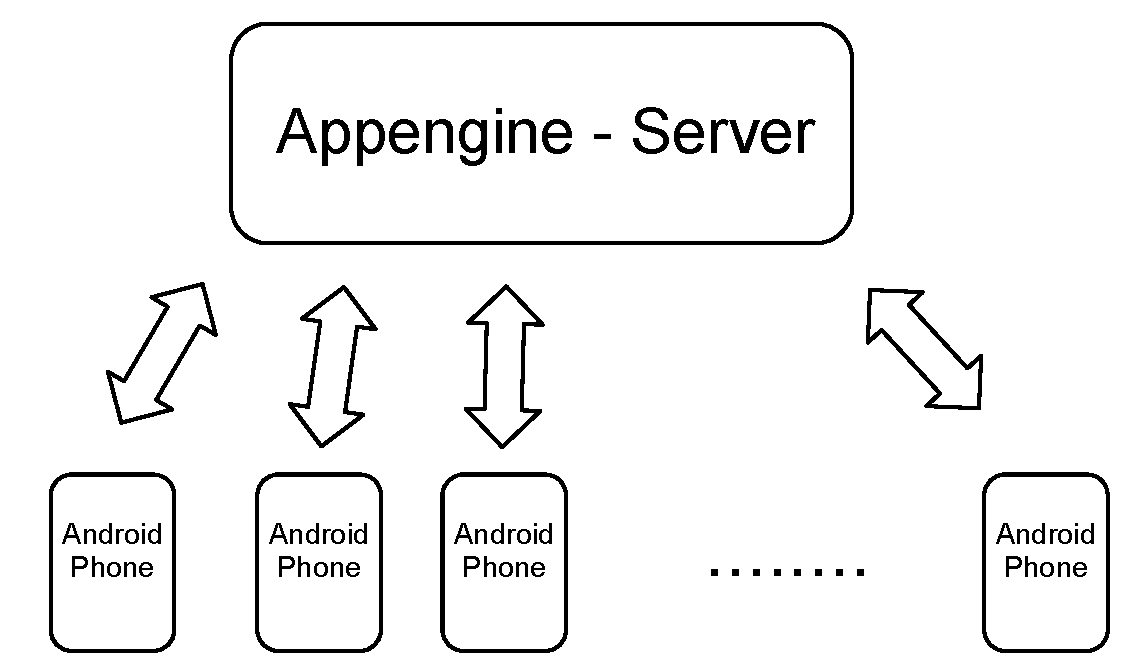
\includegraphics[scale=0.4]{figs/ServerArchitecture}
\label{fig:ServerArchitecture}
\caption{A server on Google Appenigine is used to coordinate communication between the phone clients.}
\end{figure}

\section{Measurements}
\subsection{Measuring Latency}

There are many difficulties with trying to measure latency in a distributed system.  The most naive solution would be to simply time from when one GPS reading is calculated on one phone to when that updated position is displayed on another. The problem with this, of course, is time itself is not totally ordered in a distributed system~\cite{Lamport:1978:TCO}.

\begin{figure}
\centering
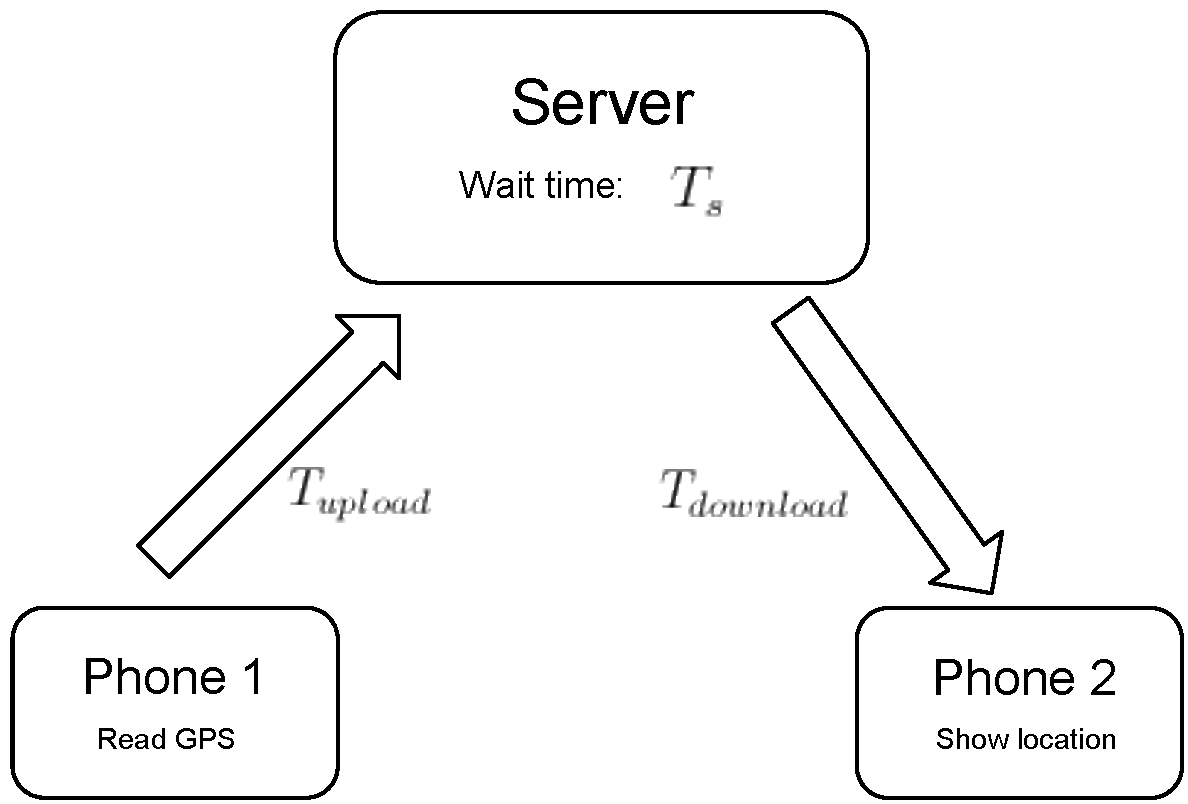
\includegraphics[scale=0.4]{figs/LatencyExplanation}
\label{fig:LatencyExplanation}
\caption{Latency can be broken down into three constituent pieces.}
\end{figure}

One solution would be to synchronize the notion of time on the phone.  If they could be synchronized within some known time bound, then we could use timestamps and have a bound on the error of that calculation.  Since phones include GPS and GPS includes a notion of time, this is a feasible solution.

Another solution would be to measure a round trip time.  It is important to make sure that the round trip time includes multiple phones, since we are interested in the time that it takes to propagate information from one phone to another.  One approach would be to time the round trip time of the following set of events.  On a single phone acquire a GPS reading, post it to the server, and then subsequently request updates of other phones' positions from the server until they change.  Under certain atomicity assumptions (namely that the reading of positions and posting of GPS update is all done in an atomic and isolated fashion) and network assumptions (that the network delivers packets in order), getting an updated position from another phone after posting your own update would be enough to guarantee that the other phone had seen the original GPS reading.  Unfortunately, this approach is complex and brittle, and many of the assumptions do not necessarily hold in practice.

A third approach is one that combines observation on the phone with observation on the server.  Rather than try to get an exact measurement of any particular point-to-point or round-trip flow of information, it merely tries to measure statistically certain subflows that can be summed up to find a statistical measure of a likely point-to-point flow.  The basic idea is that the latency for a GPS reading to move from the GPS receiver on one phone to the screen on another is made up of three parts:
\begin{enumerate}
\item the time that it takes to get from the GPS receiver on the first phone to the server,
\item the time that the reading waits on the server before it is queried by the second phone, and
\item the time that the reading takes to get from the server to the screen of the second phone.
\end{enumerate}
Since the second part is handled completely on the server, measuring it is easier than the first and third part.  The key insight for solving this problem is noticing that there is a certain degree of symmetry among the phones, especially if we average over many measurements.  It is likely that the latency for a reading to get from the server to one phone will be very close to the latency to get from the server to another.  Making this (reasonable) assumption allows us to measure the sum of the first and third parts by simply measuring the roundtrip time of two separate GPS measurements as seen by a single phone.  That is, if we assume a certain degree of symmetry among the phones, we can measure the time it takes to upload one GPS measurement and then receive a different GPS measurement from the server, and take that as a proxy for the sum of the first and third measurements.  Summing this with the time measured on the server between the GPS measurement being posted and being read by another phone gives us a very accurate overall latency for reading-to-display across multiple phones.

\subsection{Phone Simulators}
In order to get a meaningful evaluation of the entire architecture, we need to have more than just measurements of latency in the simple two-phones case.  In order to get a clear picture of how well the architecture will scale, we would like measurements of how well the system handles increasing load.  The most natural way to measure load in our system is by increasing the number of phones playing the game, but acquiring that number of hardware phones only for testing was infeasible.  Instead, we built a phone simulator that can be run on the computer and simulate the interaction of any number of phones interacting with the server. We still do the latency measurements from the real phones, since we want to take into account the potential differences in latency between 3G and Wifi connections, but phone simulators allow us to vary the load on the server in a realistic way. Since creating more players for the game also means that the real phones need to display more players on the screen, this load test is also a way of testing how efficiently the players are drawn on the screen of the handheld devices.

\subsubsection{Simulator Architecture}
The phone simulator is written in Go, and can create an arbitrary number of concurrent threads that each simulate a single phone.  Each simulated phone first queries the server requesting to join a specific game, and gets back it's player id.  It then uses that player id to generate random movement around a fixed point at a given update rate (in the examples here, we have used a 1 second update rate as that is the update rate used by the real phones). The simulator also logs all of the responses from the server and when all communications are sent and received, which would allow computation of server latency.  Since we are more interested in the server latencies for real phones, however, we do not use the simulator latencies in the results in the following section.

\subsection{Results}

\section{Conclusion}
\bibliographystyle{plain}
\bibliography{refs}
\end{document}
